% arara: lualatex
% arara: lualatex
% Typeset using lualatex

\documentclass[a4paper,10pt]{article}
\usepackage[utf8]{luainputenc}
\usepackage[pdfborder={0 0 0}]{hyperref}

\usepackage[english]{babel}

\usepackage{fouriernc}
\usepackage{tgpagella}
\usepackage{xcolor}
\usepackage[activate=true]{microtype}
\usepackage{amssymb}
\usepackage{fontspec}
\usepackage{titling}
\usepackage{titlesec}

\usepackage{calc}
\usepackage{multicol}
\usepackage{array}
\usepackage{enumitem}
\usepackage{tikz}
\usepackage{pgfplots}
\usepackage{siunitx}
\usepackage{colortbl}
\usepackage[a4paper,margin=2cm,top=1cm]{geometry}

\setmainfont[Numbers=OldStyle]{TeX Gyre Pagella}

\definecolor{plhome}{HTML}{CCEEFF}
\definecolor{silver}{HTML}{DDDDDD}

\pagestyle{empty}

\parskip=1ex
\parindent=0pt

\setlist[enumerate,1]{start=0}

\newcommand\answerspace{\\\rule[0cm]{0pt}{1cm}}

\newcommand\True{\texttt{True}}
\newcommand\False{\texttt{False}}

\newcommand\startsection[1]{
     \vspace{0.2ex}
    \hrule
    {\fontspec{Oxygen} \tiny
     \vspace{-1ex}
     \emph{#1}
     \vspace{-1.5em}
    }
}

\newfontfamily\headingfont[]{Bree Serif}
\titleformat*{\section}{\LARGE\headingfont}

\begin{document}

\section*{Blinking LED with MicroPython on ESP32}

\begin{enumerate}
\item Set up your environment. Ask booth staff for the proper handout.

\end{enumerate}

\section*{Controlling the LED}

\begin{enumerate}[resume]

\item MicroPython allows you to control the microcontroller's \emph{pins},
      to which other devices are connected.
      To do that, you need to import the \texttt{Pin} class with:

      \texttt{from machine import Pin}.

\item A pin can serve as a binary input/output.
      On the hardware side, imagine there either is electricity or there isn't.
      On the software side, you can either read \texttt{0} or \texttt{1} from an
      input pin, or write \texttt{0} or \texttt{1} to an output pin.

      Create an output Pin object for the integrated LED (\emph{Light Emitting Diode}),
      which is connected to pin \#2, and save it in a variable:

      \texttt{led = Pin(2, Pin.OUT)}

\item Write 1 or 0 to turn the light on or off:

    \texttt{
        led.value(1) \\
        led.value(0)
    }

\end{enumerate}

\section*{Blinking the LED with a button}

\begin{enumerate}[resume]

\item Let's create a program that turns the LED on when the user is holding a button.
      We'll use the integrated \emph{BOOT} button, which is connected to pin number 0.
      Create an input Pin for it:

      \texttt{~~~~button = Pin(0, Pin.IN)}

\item Read the value with \texttt{button.value()}. What is it?

\item Read the value while holding the \emph{BOOT} button. What is it?

    \textit{
        The \emph{BOOT} button is next to the USB connector.
        Don't confuse it with \emph{EN}!
    }

\item Using an infinite loop, make the LED shine if and only if you hold the button.

\item Change the program so one press of the button switches the light.
      Is there a problem? How can you check for one press?

\end{enumerate}

\section*{Blinking the LED with sleep}

\begin{enumerate}[resume]

\item Try out the \texttt{sleep} function form the \texttt{time} module.
    What does it do?

    \texttt{
        from time import sleep \\
        sleep(1/2)
    }

\item Make the LED blink 10 times with a half-second interval.

\end{enumerate}

\section*{Blinking with Pulse Width Modulation}

\begin{enumerate}[resume]

\item Make the LED blink really fast.
      On for $\frac{1}{1000}$ of a second, off for $\frac{2}{1000}$ of a second.
      What happens? What if you swap the numbers?
      This is how light intensity is usually controlled: with fast blinking.

\item Fast blinking with sleep is not very effective.
      You can use the integrated hardware \emph{Pulse Width Modulation} (PWM) instead.
      Imagine a rectangular wave as drawn here:

      % https://tex.stackexchange.com/a/113050/51382
      \begin{center}
      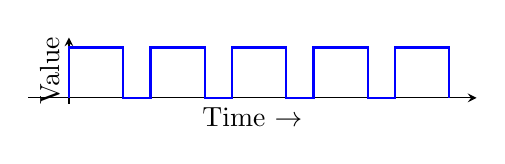
\begin{tikzpicture}
      \begin{axis}[
      width=.6\textwidth,
      height=.2\textwidth,
      x axis line style={-stealth},
      y axis line style={-stealth},
      ymax = 1.2, xmax=15,
      axis lines*=center,
      ytick={0},
      xtick={0},
      xticklabels={},
      xlabel={Time $\rightarrow$},
      ylabel={Value},
      xlabel near ticks,
      ylabel near ticks]
      \addplot+[thick,mark=none,const plot]
      coordinates
      {(0,0) (0,1) (2,0) (3,1) (5,0) (6,1) (8,0) (9,1) (11,0) (12,1) (14,0)};
      \end{axis}
      \end{tikzpicture}
      \end{center}

      A PWM will change the value of a pin from 0 to 1 and back in a periodic interval.
      The \texttt{PWM} class from the \texttt{machine} module takes 3 arguments:
      a pin, frequency and the duty cycle.

      \texttt{~~~~pwm = PWM(led, freq=50, duty=512)}

      Frequency determines how fast the LED will blink.
      Duty determines the proportion of time where the LED is on: 0 means never;
      1023 means always.
      When experimenting, mind the fact that humans don't perceive light intensity linearly.

      With a PWM running, you can do other things in Python -- it is not blocking.
      To change a PWM's frequency or duty, use the \texttt{pwm.freq(...)} or \texttt{pwm.duty(...)} methods.
      To stop a PWM, use \texttt{pwm.deinit()}.

      Try it out!

\end{enumerate}

\end{document}
